\subsection*{What class of problems is LibMesh designed to solve?}
% The ``Generic BVP'' slide has been slightly revamped for notational consistency
\begin{frame}[t]
  %\frametitle{A Generic BVP}
  \begin{columns}[t]
    \column{.5\textwidth}
     \begin{itemize}
      \item General boundary value problems of the form:
      \end{itemize}
%    \begin{block}{}%{We assume there is a Boundary Value Problem of the form}
      \vspace{-.1in}
        \begin{eqnarray}
	\label{eqn:general_pde}
	\nonumber
	M \frac{\partial u}{\partial t} & = & F( u ) \;\;\;\; \in \Omega
        \\
	\nonumber
	G( u ) & = & 0 \;\;\;\;\;\;\;\;\; \in \Omega
	\\
	\nonumber
	u & = & u_D \;\;\;\;\;\;\; \in \partial \Omega_D
	\\
	\nonumber
	N(u) & = & 0 \;\;\;\;\;\;\;\;\; \in \partial \Omega_N
 	\\
 	\nonumber
 	u(\bv{x}, 0) & = & u_0(\bv{x}) 
      \end{eqnarray}
%    \end{block}
    %\pause
    \column{.5\textwidth}
      \begin{center}
	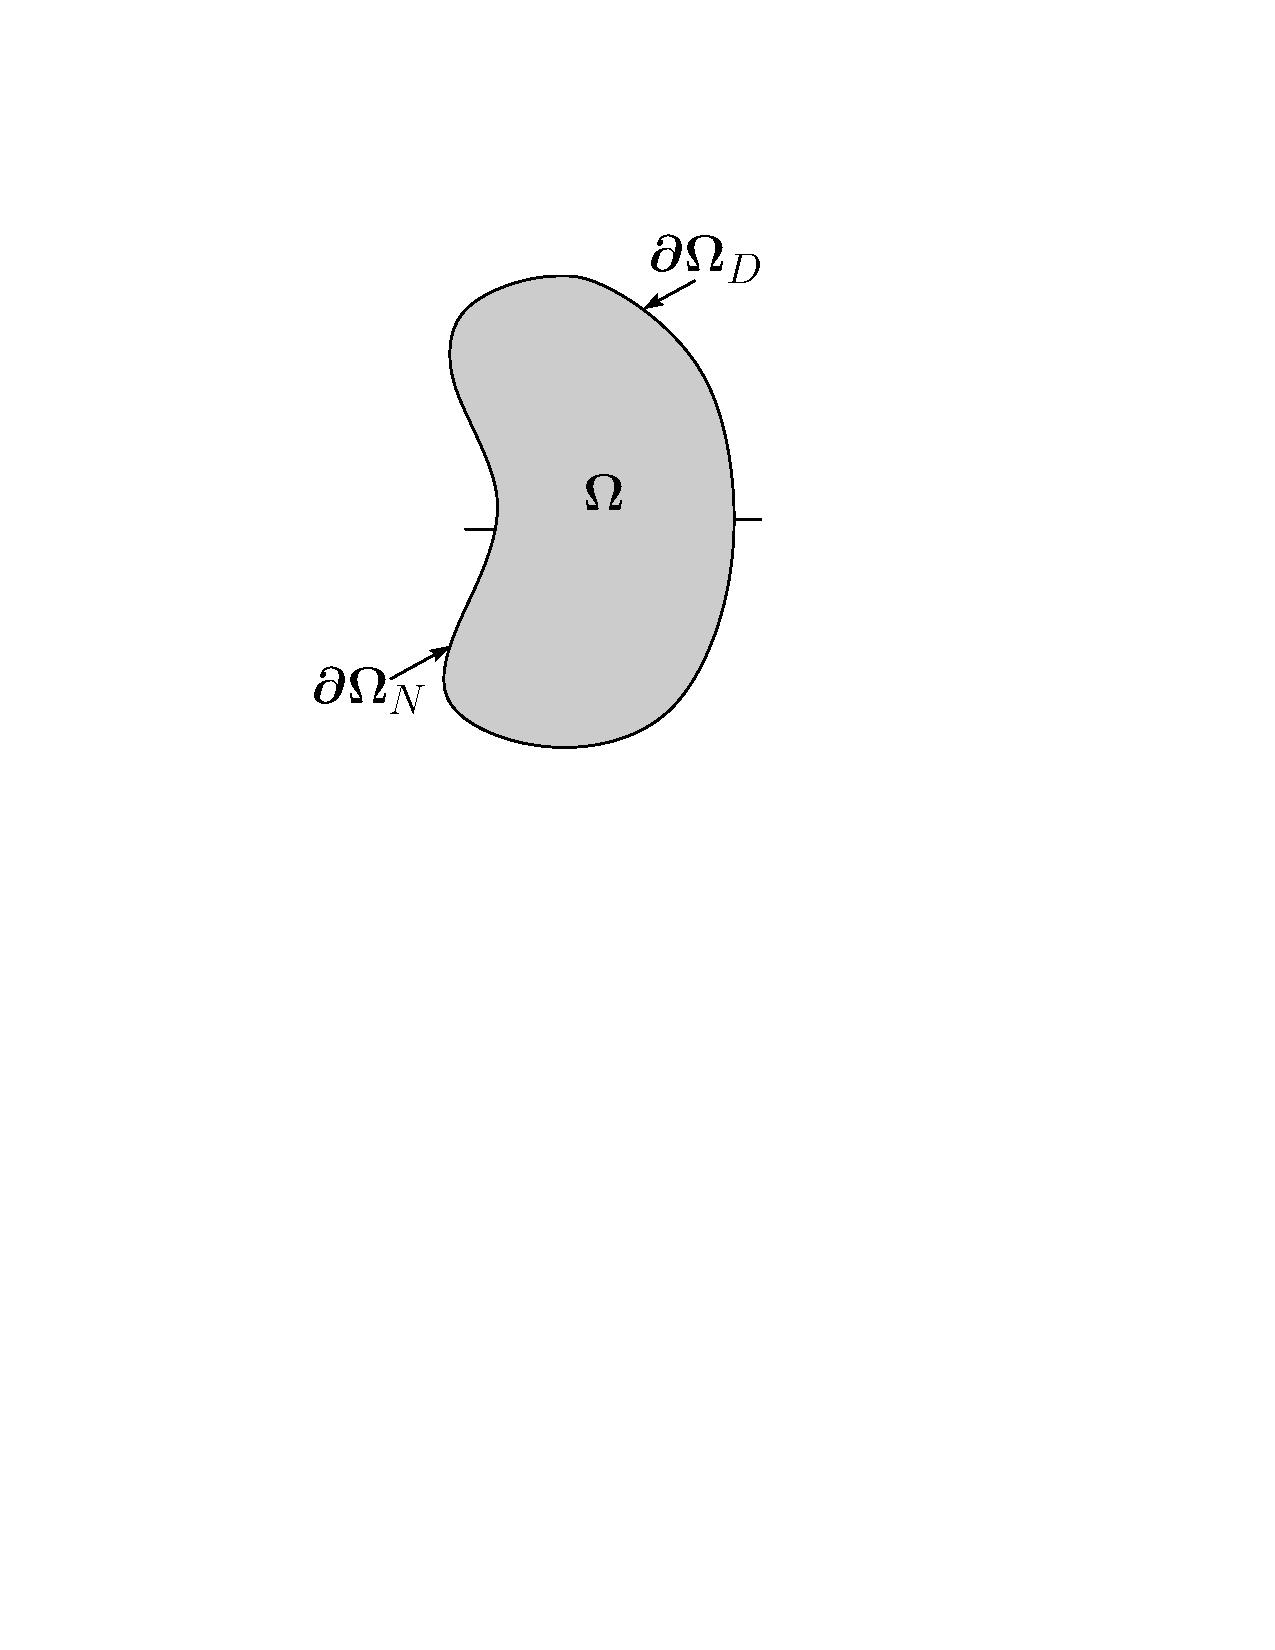
\includegraphics[viewport=140 420 400 685,clip=true,width=2in]{figures/domain2/domain2_input}
      \end{center}
  \end{columns}
\end{frame}
